% Topical subheadings are allowed. Authors must ensure that their Methods section includes adequate experimental and characterization data necessary for others in the field to reproduce their work.

\section*{Methods}
\label{sec:methods}
% \note{3000 words limit.}

% To ensure the correct interpretation of the results presented in this article, it is important to understand the implementation details of the NeuroBench harness. This section will elaborate upon the metrics, tasks and baselines included in the algorithmic track. Next to that, the metric calculations used within the system track and the QUBO system track benchmark are explained.

This section outlines details and specifications of the benchmark metrics, tasks, and baselines.

\subsection*{Algorithm Track Metrics}

% \JY{Should we get rid of the implementation notes such as nn.modules, layers supported? If this is read far into the future there will be expanded support. Could say something like updated details are available on the repo?}

NeuroBench includes correctness and complexity metrics, the latter of which is divided in static and workload metrics. Static metrics do not depend on the model inference and input data, while the workload metrics do. Note that the defined metrics reflect only the model and model execution. Data pre-processors and post-processors are not taken into account in the v1.0 algorithm track results. 
% The harness currently supports the use of PyTorch \texttt{nn.Modules}.
% other layer types or activation functions can be added with the provided functions of the \texttt{NeuroBenchModel}.

\subsubsection*{Footprint}
The footprint metric reflects the memory footprint a model. It is distinct from execution memory, which may incur further usage, e.g. to store activations. It is computed for a model by accumulating the sizes of the model's parameters and buffers, in bytes.
% These buffers are important to take into account when the model stores tensors which do not require a gradient. 
Parameters store the model synaptic weights, and buffers include other inference memory requirements, such as the internal states of recurrent or spiking layers and buffers of recent input data, if the model must record data for input binning. Considering $n$ parameters, each requiring $p_i$ bytes, and $b$ buffers of size $q_j$, the total model footprint is $\sum_{i=0}^{n}p_i + \sum_{j=0}^{b}q_j$.

\subsubsection*{Model Execution Rate}
Execution rate is a numeric which is not directly computed by the harness, but should be reported by the user. 
The numeric reflects the real-time correlation of the rate at which the model computes input data. If the model processes input with a temporal stride of $t$~seconds, then the rate should be reported as $t^{-1}$~Hz. Note the distinction between \textit{stride} and \textit{bin window} - input can be binned in overlapping windows, but execution rate depends on the temporal stride of window processing. As an example, a model may use 50~ms windows of input and compute every 10~ms, which would give an execution rate of 100~Hz.

This numeric is currently not well-defined for models operating under event-based or continuous-time contexts. These limitations will be addressed in future benchmark versions.
% as needed to support research and tools facilitating such methods.

\subsubsection*{Connection sparsity} 
The parameter matrices of each layer $l$ in a model, representing synaptic weights, are collected, and the number of zero weights $m_l$ and total weights $n_l$ are aggregated, with the connection sparsity defined as $\frac{\sum_l m_l}{\sum_l n_l}$.

% For each layer ($l$), each weight matrix ($W_l^i$) is collected, and the numbers of zero weights ($m_{l}^i$) and total number of weights ($n_l^i$) of each weight matrix $i$ are accumulated.
% % Across all weight matrices within a layer, and all layers, the number of zero weights and number of weights are accumulated. 
% The connection sparsity of the model is the complement of the ratio of the zero weights over total weights, 
% $1 - \sum_l \frac{(m_l)}{(n_l)}$.

% The layers currently supported by the harness are: \texttt{nn.Linear}, \texttt{nn.Conv1d}, \texttt{nn.Conv2d}, \texttt{nn.Conv3d}, \texttt{nn.RNN}, \texttt{nn.RNNBase}, \texttt{nn.RNNCell}, \texttt{nn.GRU}, \texttt{nn.GRUBase}, \texttt{nn.GRUCell}, \texttt{nn.LSTM}, \texttt{nn.LSTMBase}, \texttt{nn.LSTMCell}.


\subsubsection*{Activation sparsity}
Activation sparsity is computed after the inference phase. The sparsity is calculated by accumulating the number of zero activations ($z$), over all neuron layers ($l$), timesteps ($t$), and input samples ($i$) and dividing by the total number of neurons ($N$), $\frac{\sum_l \sum_t \sum_i z_{l,t}^i}{\sum_t \sum_l \sum_i N_{l,t}^i}$. 
The outputs of ReLU functions and spikes from spiking neurons are considered activations.
% The included activation types are \texttt{nn.ReLU, nn.Sigmoid, nn.Tanh} and all snnTorch neurons that are subclasses of \texttt{NeuronModel}. Custom activations can be added before running the benchmark by using the \texttt{NeuroBenchModel.add\_activation\_module} function.

\subsubsection*{Synaptic operations}
% \TODO{Note about \textit{Dense} vs \textit{EFF\_MACs} vs \textit{EFF\_ACs}}
Synaptic operations are the multiplication of weights by activation or input data, and are calculated using the inputs and weights of connection layers (e.g., \texttt{torch.nn.Linear} and \texttt{torch.nn.Conv2d}).
Effective synaptic operations are operations where a non-zero weight is multiplied by a non-zero activation. 
% The reasoning behind this definition is that specialized hardware can make use of the sparsity in the input and weight matrices, representing the synapses. 
% The metric distinguishes between the effective multiply-accumulates (MACs) in normal layers,  effective accumulates (ACs) in binary layers, and the total dense operations, which represents the number of MACs required when computed on conventional hardware. 
Effective operations are further divided into multiply-accumulates (MACs), and accumulates (ACs), where accumulates correlate with activations or input data only containing values of [-1, 0, 1], and multiply-accumulates cover all other cases.
The reported number of synaptic operations is the average number of synaptic operations required per model execution, the rate of which is defined by the \textit{model execution rate} metric.

% input sample, when a sample is well-defined and independent such as in a classification task. In continuous tasks such as time-series modeling and continuous detection, the metric reports average operations per model computation, the rate of which is defined by the 
% % Frequency metric.
% Execution Rate metric.

% Therefore, this is an accumulated metric. Meaning that the number of MACs and ACs are accumulated throughout the benchmark and normalized to a single sample at the end. 

The number of \textit{effective} synaptic operations is computed by performing the forward pass of a layer and counting the number of operations in which there is no zero multiplication.
Practically, this is implemented in the harness by setting all non-zero weights in the layer and all the non-zero activations to 1, then performing the forward pass and summing the output to give the number of synaptic operations. 

% This is demonstrated below for a linear layer. Assume the bias to be zero, resulting in a forward pass following $y=W\cdot x$. An example weight and activation vector is presented below.\\
% \begin{equation}
%     W\cdot x=
%     \begin{bmatrix}
%         1.3 & 0 & -3.2 \\
%         0 & 1.2 & -5.1 \\
%         -1.1 & 2.7 & 0 \\
%      \end{bmatrix}    \cdot \begin{bmatrix}
%          0 \\
%          1.3 \\
%          -1 \\
%      \end{bmatrix} 
% \end{equation}
% Both the weight matrix and the activation vector contain zeroes, so effective synaptic operations are only performed for a subset of the weight and input combinations. We make the weight matrix and input matrix binary and compute the forward pass to yield effective operations.
% \begin{equation}
%      \begin{bmatrix}
%         1 & 0 & 1 \\
%         0 & 1 & 1 \\
%         1 & 1 & 0 \\
%      \end{bmatrix}    \cdot \begin{bmatrix}
%          0 \\
%          1 \\
%          1 \\
%      \end{bmatrix} = 
%      \begin{bmatrix}
%          1 \\
%          2 \\
%          1 \\
%      \end{bmatrix} \rightarrow 
%      SynOps = 4
% \end{equation}

The number of \textit{dense} synaptic operations is computed in a similar fashion, by setting all weights and activations to 1 and accumulating the output of the forward pass.
Biases are not taken into account in the calculation of the synaptic operations, as they are added after weight multiplications and accumulation. 

Note that processing of activations before the connection layer, for instance using batch normalization, can transform sparse activations into dense input at the connection layer, which will lead to high effective synaptic operations despite high activation sparsity. Furthermore, such processing can transform binary activations to non-binary data, causing effective operations to be MACs rather than ACs. When deployed to neuromorphic hardware, such algorithms that normalize activations before multiplication with synaptic weights may lose the benefits of sparse operation, e.g., an SNN with normalization following each spiking layer would require dense MAC weight calculation, no matter how few spikes were generated.

In some cases, algorithm execution may have distinct temporal sections of higher and lower synaptic operations, such as during initial caching versus continuous inference. For such algorithms, benchmark users may choose to distinguish synaptic operations and other complexity measurements between execution sections.

% Accumulating the number of effective synaptic operations $SynOps$ for each layer gives the total effective synaptic operations required. Depending on whether the input $x$ is binary, which is the case for non-graded SNN, or non-binary, the effective operations are classified as ACs or MACs respectively. Next to the effective synaptic operations, the dense synaptic operations are reported, where the number of synaptic operations consisting of zero multiplications is also taken into account.

% Additional metrics are currently implemented in algorithm track harness. An example is the number of updates per neuron type. This metric returns the number of times each neuron type was updated. For this metric, it is assumed that the neuron is only updated when a non-zero signal is passed. 

\subsection*{Algorithm Track Benchmark Tasks}
\subsubsection*{Keyword FSCIL}
Few-shot Class-Incremental Learning, FSCIL, is an established benchmark task setting in the computer vision domain~\cite{tao2020fscil}. It can be defined as follows: a base session with fixed classes, each with abundant training data, is used to train an initial model. Then, successive incremental training sessions introduce new classes in a few-shot learning scenario. In each session, only the current session classes are available to the model for training. After each incremental training session, the model is evaluated on all previously seen classes, including the base classes. Therefore, the model has to learn new classes while retaining knowledge about the previously learned ones. 

Formally, for $M$-step FSCIL, where $M$ is the total number of incremental sessions, each training session uses a support dataset $D^{(t)}$, $t\in [0,M]$ to train new classes on. ${L^{(t)}}$ is the set of classes of the $t$-th session where $\forall i,j$  where $i \neq j$, $L^{(i)}\cap L^{(j)}=\varnothing$, meaning each training session uses a unique set of classes. $D^{(0)}$ and $L^{(0)}$ are the base class training data and set of base classes, respectively, $D^{(1)}$ and $L^{(1)}$ represent the first incremental session set, and so on. At session $t$, only $D^{(t)}$ is available for training, and for $t>0$, $D^{(t)}$ contains a fixed number of classes ($N$) with few samples per class ($K$). This form of FSCIL is therefore named $N$-way $K$-shot FSCIL. At the end of each session $t$, model accuracy is reported on the test samples of all previously seen classes $\{L^{(0)} \cup L^{(1)} \cup ... \cup L^{(t)}\}$.

% \TODO{We have formalism of dataset, but not yet formal problem setup description: https://arxiv.org/pdf/2304.08130.pdf}

For the Keyword FSCIL task, classes in the base set ($L^{(0)}$) have 700 samples each, with a fixed train/validation/test sample split of 500/100/100. All classes within incremental sessions have 200 samples per word, with a fixed train/test split of 100/100. Of the 100 training samples, 5 are randomly selected for few-shot learning (each session is 10-way, 5-shot). The inclusion of 200 samples allows for increasing learning up to 100 samples. 


NeuroBench proposes an audio keyword classification version of the FSCIL task, which to the best of our knowledge is the first of its kind. This novel task is established by selecting a subset of the words and languages from the Multilingual Spoken Word Corpus (MSWC)~\cite{mazumder21mswc} dataset. The FSCIL task consists of a multilingual set of 100 base classes and 10 incremental sessions of 10 classes each, for a final total of 200 learned classes. 
% To increase the diversity of demographics represented by the dataset, multiple languages, covering multiple language families, are included. 
% A set of 5 base languages with 20 words each and 10 incremental languages with 10 words each was chosen, based on the data availability. 
Fifteen languages are represented: the base classes are composed of a set of five base languages with 20 words each, and each of the ten incremental sessions contains 10 words from a distinct language. The languages were chosen based on data availability within the MSWC dataset. The top five languages with the greatest number of potential words (words with enough data samples) are used as the base class languages, while the next ten languages with the greatest numbers are the incremental classes. 
The base languages are English, German, Catalan, French and Kinyarwada. Incremental languages are Persian, Spanish, Russian, Welsh, Italian, Basque, Polish, Esparanto, Portuguese and Dutch. The order of languages presented in the incremental sessions are randomized, but each incremental session will represent exactly one new language.

For each language, the longest length words (that had the appropriate number of samples) were selected to allow for rich and robust temporal features to be learned. Next to the richness of longer words, there are practical considerations for this choice. The MSWC dataset normalizes all samples to a duration of 1 second, centered around the 0.5 seconds mark. For shorter words, this means that the data needs to be zero-padded on both sides to fill the entire duration. Longest-length words are likely to fill the complete sample and reduce zero-padding, which is also useful in scenarios in which algorithms seek to classify words before the sample has completed~\cite{jeffares2022spikeinspired}. Furthermore, common keyword spotting solutions, such as \textit{Ok Google}, \textit{Alexa}, and \textit{Hey Siri}, use multi-syllable wake-phrases to assist in accurate word classification. \revision{Using shorter keyword subsets can lead to greater challenge in both base language training and continual class learning. The full list of chosen words for the task presented in this paper (longest words), as well as other potential subsets of short words for the same languages, can be found with dataset documentation through the harness.}

Within each language, words showing great similarity in phonics and meaning are not included (e.g. l'amendement and amendements in French). Across different, but related languages, words with similar pronunciation and meaning were not included as well (e.g., university, universität and universitat in English, German and Catalan).

The subset of MSWC used for this FSCIL task is significantly smaller in size (630MB) compared to the full MSWC datatset (124GB), and subset download details can be found in the harness.

% \TODO{Where to download the subset of the dataset}
% The subset of the original dataset, which is used in this task, is hosted by NeuroBench. A complete list of the words used for this task, and the relevant download instructions, can be found in the \red{documentation}.

\subsubsection*{Event Camera Object Detection}
The task of object detection using event camera data involves identifying bounding boxes of objects belonging to multiple predetermined classes in an event stream. The dataset is the Prophesee 1 Megapixel automotive detection dataset~\cite{Perot2020}, which is one of the largest and highest-resolution event-camera detection datasets currently available. The performance of the task is defined by the COCO mean average precision (mAP) metric~\cite{LinCOCO_2014}, a metric that is commonly used for the evaluation of object detection algorithms. Only three out of the seven available object classes within the dataset are used due to limited sample availability in the dataset, which matches prior work~\cite{Perot2020}.

COCO mAP is calculated using the intersection over union (IoU, Equation~\ref{eq:iou}) of the bounding boxes produced by the model against ground-truth boxes. Here, $A$ and $B$ refer to bounding boxes, and the intersection and union consider the overlapping area and the area covered by both boxes, respectively. The IoU is compared against 10 thresholds between 0.50 and 0.95, with a step size of 0.05.
For each threshold, precision is calculated (Equation~\ref{eq:precision}) with True Positives (\textit{TP}) and False Positives (\textit{FP}) determined by whether the IoU meets the threshold or not, respectively. The mAP is calculated as the averaged precision over all thresholds for each class, which is further averaged over all classes to produce the final result.

\begin{equation} \label{eq:iou}
    IoU(A,B) = \frac{|A\cap B|}{|A\cup B|}
\end{equation}

\begin{equation} \label{eq:precision}
    Precision(TP,FP) = \frac{\sum TP}{\sum TP + \sum FP}
\end{equation}

% COCO mAP specifies the threshold selection of the intersection over union (IoU) to be a series of 10 thresholds between 0.50 and 0.95 with a step size of 0.05. The calculation of the mAP consists of multiple steps. First, the model detects the relevant objects and provides a bounding box and class label. Then, the IoU for each detection is computed, which represents the overlap of the predicted bounding box, $A$, versus the correct bounding box $B$:

% For all IoUs, we compare to each of the 10 COCO thresholds. If this is higher than  the threshold, the prediction is classified as a True Positive, \textit{TP}, else it is a False Positive, \textit{TF}. From these, we can calculate the average precision, and subsequently, th mean average precision (mAP). 

Note that in the dataset, labels are generated from images from an RGB camera. Due to the nature of event cameras, objects which are still at the start of a recording sequence have no generated events and cannot be detected. Therefore, labels within the first 0.5 seconds of each sequence are not taken into account. Furthermore, as the RGB camera used for labeling has a higher resolution than the event camera, not all objects which appear in the RGB image are recognizable from the generated events. Thus, objects with a diagonal of less than 60 pixels are also not considered. The dataset and metric measurement is implemented using the Prophesee Metavision software~\cite{metavision}.
%3) IoU Threshold Selection: On COCO, the average precision is evaluated over several IoU values, the thresholds of 0.50, the range 0.50-0.95, and 0.75. 

% The object detection benchmark utilizes the Prophesee 1 Megapixel Automotive Detection Dataset. This dataset was recorded with a high-resolution event camera with a 110 degree field of view mounted on a car windshield. The car was driven in various areas under different daytime weather conditions over several months. The dataset was labeled using the video stream of an additional RGB camera in a semi-automated way, resulting in over 25 million bounding boxes for seven different object classes: pedestrian, two-wheeler, car, truck, bus, traffic sign, and traffic light. The labels are provided at a rate of 60Hz, and the recording of 14.65 hours is split into 11.19, 2.21, and 2.25 hours for training, validation, and testing, respectively. For the data included in NeuroBench, three classes are included, namely car, pedestrian and two-wheelers. These occur far more often in the recorded data than the remaining classes. Next to that, prior work included the three aforementioned classes. 


\subsubsection*{Non-human Primate Motor Prediction}
% The non-human primate motor prediction task is a predictive modeling task. Using neural data from the sensorimotor cortex, the task is to forecast the horizontal and vertical fingertip positions, x and y respectively. The metric used to measure the accuracy of the prediction is the $R^2$-score. Which is computed given the correct fingertip positions $X_i,Y_i$ and the predicted fingertip positions $x_i,y_i$, for across $n$ predictions. 
The non-human primate motor prediction task involves predictive modeling of two-dimensional fingertip velocity, given neural motor cortex data.
The six sessions used for the benchmark comprise three recording sessions each from two non-human primates (NHP Indy and NHP Loco) such that the chosen sessions approximately span the entire duration of the experiment~\cite{makin-dataset} (several months).
The specific sessions used are indy\_20170131\_02, indy\_20160630\_01, indy\_20160622\_01, loco\_20170301\_05, loco\_20170215\_02, and loco\_20170210\_03.
Each of these sessions consists of one day of experiments, during which multiple reaches are recorded. During each reach, a target position is displayed, which the NHP needs to localize and touch with its finger. Once the NHP touches the correct target for the current reach, the next reach is instantiated, showing a new target position. The data contains sensorimotor cortex recordings from 96 channels for the recordings of the first NHP (Indy), while 192 channels were used for the second NHP (Loco), and was gathered and labeled at a frequency of 250Hz. Two-dimensional position data of the NHP fingertip during its reaches is provided in the dataset, and these are translated into $X$ and $Y$ velocity ground-truth labels using discrete derivatives~\cite{makin-paper}.

Each session is segmented into individual reaches based on the target position for the NHP to touch. 
The data in each session is split such that the initial $75\%$ of reaches are used for training and validation, and the remaining $25\%$ of reaches are test data. The user can choose how to utilize the training and validation split for their particular method.  

During evaluation, the coefficient of determination ($R^2$, Equation~\ref{eq:r2}) for the $X$ and $Y$ velocities are averaged to report the correctness score for each session, where $n$ is the number of labeled points in the test split of the session, $y_i$ is the ground-truth velocity, $\hat{y_i}$ is the predicted velocity, and $\bar{y}$ is the mean of the ground-truth velocities. The $R^2$ from sessions for each NHP are averaged, producing two final correctness scores.

\begin{equation} \label{eq:r2}
    R^2 = 1 - \frac{\sum_{i=1}^{n} (y_i - \hat{y_i})^2}{\sum_{i=1}^{n} (y_i - \bar{y})^2}
\end{equation}

\subsubsection*{Chaotic Function Prediction}
% Similarly to the non-human primate motor prediction task, the Mackey Glass function prediction is a sequence-to-sequence problem, meaning that given an input sequence, the task is to predict the future values of the same function, $y(t)=x(t)$. Input data is passed to the model at an interval of $\Delta t$, given the history, the model expected to predict the  next point. After an entire run, the model will have made a prediction $y(t)$ of the original function $x(t)$. Subsequently, the Mean Squared Error (MSE) is used to measure the accuracy of the model across the entire run. 

The chaotic function prediction is another sequence-to-sequence problem. Given an input sequence generated from a one-dimensional Mackey-Glass function, the task is to predict the future values of the same function.
The dataset used for this task is synthetically generated, following the Mackey-Glass differential equation~\cite{mackey1977oscillation} (Equation \ref{eq:MackeyGlass}), which is integrated and discretized with a timestep of $\Delta t$. The time series generated by this differential equation is a function of the Mackey-Glass parameters $n$, $\beta$, $\gamma$ and $\tau$. Adhering to standard parameters~\cite{jaeger2004harnessing}, the values used for $n$, $\beta$, and $\gamma$ are 10, 0.2 and 0.1 respectively. $\tau$ is varied between 17 (a standard value) and 30, leading to 14 time series which vary greatly in dynamics and can be used to analyze the generalization of predictive models.

Each value of $\tau$ is associated with a Lyapunov time, the expected predictability timescale for chaos~\cite{gilpin2023largescale}, which is used as the time unit for each series. To calculate the overall Lyapunov time for each value of $\tau$, we average the Lyapunov times of 30,000 generated time series of 2,000 timesteps, with $\Delta t=1.0$, each with a randomly chosen initial condition.
All time series and Lyapunov times were generated and estimated using the \texttt{JiTCDDE} library~\cite{jitcxde}. 
For each final time series used for benchmarking, initial conditions are a point randomly chosen along the series.
The Lyapunov time and initial condition $x_0$ for each of the 14 final time series are provided in Table \ref{tab:MG_params}.

% For each value of $\tau$, the Lyapunov time is computed to be the nearest whole number by averaging over 30,000 generated time series of 2,000 timesteps ($\Delta t=1.0$), each with a randomly chosen initial condition where the Lyapunov time for individual time series is estimated by the \texttt{JiTCDDE} library~\cite{jitcxde}.  
% Initial conditions for each final time series is a point randomly chosen along the series.
% The Lyapunov time and initial condition $x_0$ for each of the 14 values of $\tau$ are provided in Table \ref{tab:MG_params}.

\begin{equation} \label{eq:MackeyGlass}
    \frac{dx}{dt} = \frac{\beta x(t-\tau)}{1 + x(t-\tau)^n} - \gamma x(t)
\end{equation}

% Within NeuroBench, Mackey Glass series for 14 sets of parameters (varying $\tau$, Lyapunov time and $x_0$) are provided (table \ref{tab:MG_params}). A large range of different values for $\tau$ allow the user to analyze the robustness of their algorithm for the different settings. For every set of parameters, the datasets are precomputed to avoid variability between systems due to low-level libraries solving differential equations. The differential equation solver relies on the \texttt{jitcdde} library, which can produce different output on different machines based on platform microarchitecture. For computing this differential equation, integration parameters have to be defined. Firstly, the absolute error tolerance, which determines the maximum error between the prediction and the analytical solution of the differential equation, is defined. When the error is larger than this parameter, the timestep gets reduced. Related to the absolute tolerance is the relative tolerance. Where the absolute tolerance takes the difference between the prediction and the exact result, the relative tolerance takes the difference and divides by the magnitude of the exact solution. As the step size may become very small when solving the differential equation, cohering to the aforementioned parameters, a minimum step size is defined to avoid unnecessarily long computations. \KVDB{add exact values}. Using these integration parameters, timeseries for every combination of parameters in table \ref{tab:MG_params} are generated, all using the Mackey Glass parameters where $n$ is 10, $\beta$ is 0.2 and $\tau$ is 0.1. The length of the timeseries is 50 times the respective Lyapunov time, each with 75 data points per Lyapunov time, ensuring enough data to train, validate and test the model with varying time offsets. The instructions on retrieving this dataset can be found in the \texttt{MackeyGlass} dataloader included in NeuroBench.

As the integration of the differential equation can depend on underlying floating-point arithmetic and thus produce varying time series on different machines, the datasets are precomputed and loaded for training and evaluation. In the benchmark results, 30 instantiations of the Mackey Glass system are used, each with a length of 20 Lyapunov times and successively shifted forwards by half a Lyapunov time. The dataset time series are generated for 50 total Lyapunov times to allow for varied offset starting points. The generated time series are available to be downloaded under the NeuroBench harness.

\begin{table}[ht]    
    \begin{center}
    \begin{tabular}{|c|c|c|}
        \hline
        $\tau$ & Lyapunov Time & $x_0$ \\ \hline
        17 & 197 & 0.7206597 \\
        18 & 138 & 0.7744313 \\
        19 & 315 & 0.7783468 \\
        20 & 131 & 0.9225991 \\
        21 & 191 & 0.9479431 \\
        22 & 119 & 0.5455960 \\
        23 & 106 & 0.8622247 \\
        24 & 97 & 0.3259660 \\
        25 & 98 & 0.8297825 \\
        26 & 104 & 1.0033490 \\
        27 & 112 & 0.6491406 \\
        28 & 119 & 1.0957495 \\
        29 & 131 & 0.9256179 \\
        30 & 139 & 0.2713639 \\
        \hline
    \end{tabular}
    \end{center}
    \caption{Mackey-Glass parameters used for the 14 time series.}
\label{tab:MG_params}
\end{table}

Symmetric mean absolute percentage error (sMAPE, Equation~\ref{eq:smape}), a standard metric in forecasting~\cite{MAKRIDAKIS202054}, is used to measure the correctness of the model predictions $\hat{y_i}$ against the ground-truth $y_i$, over $n$ data points in the test split of the time series. 
The sMAPE metric has a bounded range of $[0, 200]$, thus diverging predictions (infinity or NaN) due to floating-point arithmetic have bounded error which can be used to average correctness over multiple time series instantiations.

\begin{equation} \label{eq:smape}
    sMAPE = 200 \times \frac{1}{n} \left( \sum_{i=1}^{n} \frac{|y_i - \hat{y_i}|}{(|y_i| + |\hat{y_i}|)}\right)
\end{equation}

\subsection*{Algorithm Track Baselines}
% This section details the baseline methods implemented for each task. \TODO{Training details were commented out from main text, make sure they are added here.}

All baselines are implemented using PyTorch \texttt{nn.Module} objects in order to interface with the harness.

\subsubsection*{Keyword FSCIL}

The ANN baseline employs Mel-frequency cepstral coefficients (MFCC) pre-processing along with a modified version of the M5 deep convolutional network architecture~\cite{dai2016deep}. 

The MFCC pre-processing converts the 48~kHz, 1~second audio samples from MSWC into 20 channels of 200 timesteps (5~ms stride, 10~ms time bins), focusing on frequencies within the human voice range between 20~Hz and 40~kHz.
The network contains four successive blocks, each consisting of 1D convolution, batch-normalization, ReLU activation, and max-pooling layers, followed by a single readout fully-connected layer. Convolutional layers apply their kernels over the temporal dimension of the samples, thus extracting longer temporal features through the depth of the network. 
We also incorporate dropout after the ReLU activations to avoid over-fitting and let the network be more general for incremental learning. 
% The detailed parametrization of this modified M5 network can be found in the neuroBench repository.   
The network is trained with stochastic gradient descent using cross-entropy loss and the Adam optimizer.


For the SNN baseline, we employ the Speech2Spikes~\cite{stewart23speech2spikes} (S2S) preprocessing algorithm to convert audio samples to spikes.
For S2S we use the default parameters from the original implementation, only the hop length is updated to match the 48~kHz audio frequency of the MSWC samples, whereas the original implementation was applied to 16~kHz audio. S2S applies a Mel Spectrogram and a log operation to raw audio samples, converting them to positive and negative trains of spikes using delta-encoding.

Spike trains from S2S are used as input for the recurrent SNN (RSNN), which consists of 2 recurrent adaptive leaky integrate-and-fire (RadLIF) layers of 1024 neurons and one linear output layer. The model architecture is adapted from Bittar's work~\cite{bittar22surrogate}.
The RadLIF neurons in these layers are LIF neurons that produce a binary spike $\mathbf{s}(t)$ and reset via subtraction when their membrane potential $\mathbf{u}(t)$ crosses a certain threshold value $\theta$, combined with an extra adaptation variable $\mathbf{w}(t)$ to enable more complex temporal dynamics and firing patterns. Equation~\ref{eq:adLIF_current} is the input current to neurons, with $x$ the input spikes from the previous layer, $W_f$ the forward weight matrix, $BNTT$ batch-normalization through time, and $W_r$ the recurrent weight matrix. $\mathbf{u}(t)$ and $\mathbf{w}(t)$ are shown in Equation~\ref{eq:adLIF}, where $\alpha$, $\beta$, $a$ and $b$ are heterogeneously trainable parameters of the neuron. Finally, spikes $\mathbf{s}(t)$ are generated according to Equation~\ref{eq:adLif_spike}.

\begin{equation} \label{eq:adLIF_current}
    \mathbf{I}(t) = BNTT(W_f[x(t)]) + W_r[s(t-1)]
\end{equation}


\begin{equation}
    \label{eq:adLIF}
    \begin{aligned}
        \mathbf{u}(t) &= \alpha \left[ \mathbf{u}(t - 1) \right] + (1 - \alpha)\left[\mathbf{I}(t) - \mathbf{w}(t - 1)\right] - \theta [\mathbf{s}(t - 1)] \\
        \mathbf{w}(t) &= \beta [\mathbf{w}(t - 1)] + a (1 - \beta)  [\mathbf{u}(t - 1)] + b [\mathbf{s}(t - 1)] \\
    \end{aligned}
\end{equation}

\begin{equation} \label{eq:adLif_spike}
    \mathbf{s}(t) = 
    \begin{cases}
        0 \text{ if } \mathbf{u}(t) < \theta \\
        1 \text{ if } \mathbf{u}(t) \geq \theta
    \end{cases}
\end{equation}

% where $\alpha$, $\beta$, $a$ and $b$ are heterogeneously trainable parameters of the neuron. $I(t) = BNTT(Wx(t)) + Vs(t-1)$ is the input current to the neuron, with $x$ the input spikes from the previous layer, $W$ the forward weight matrix, $BNTT$ a batch-normalization through time and $V$ the recurrent weight matrix. Output spikes are also passed through a dropout layer. 
The last layer of the network is a readout linear classifier, and the class corresponding to the maximum of the summation of output activities over all timesteps is chosen as the network prediction.
The RSNN network is trained with backpropagation through time using a boxed pseudo-gradient and cross-entropy loss.


\begin{center}
\begin{minipage}{.9\linewidth}
\begin{algorithm}[H]
\caption{Few-Shot Class-Incremental Learning with Prototypes}
\label{alg:prototypical_continual_learning}
\textbf{Requires:} Pre-trained network $g \circ f$ consisting of feature extractor $f$ and classifier $g: x 	\mapsto Wx+b$ \\
\textbf{Define:} $(x)_l$, $w_l$ and $b_l$ respectively the set of input samples, classifier weights and biases associated with a class $l$
\begin{algorithmic}[1]
\For{each base class $k$}
\State Compute prototype embedding $c_k = \text{Mean}[f((x)_k)]$ ~~~~~~~~~~~~~~~~ \textit{(also summed over time for SNN baseline)}
\State Compute corresponding classifier weights $w_k = 2c_k$ and biases $b_k = - c_kc_k^T$
\EndFor
\State Replace classifier layer $g$ with prototype weights: $W \leftarrow W_{B} = (w_k)_{k \in B}$ and biases $b \leftarrow b_{B} = (b_k)_{k \in B}$
\For{each session $i$ in sessions}
    \State Get session support $S^i$
    \State Repeat lines \textit{1} to \textit{4} for all new classes of $S^i$ to get prototype weights $W_{S^i}$ and biases $b_{S^i}$
    \State Extend the classifier layer weights $W \leftarrow [W, W_{S^i}]$ and $b \leftarrow [b, b_{S^i}]$
\EndFor
\end{algorithmic}
\end{algorithm}
\end{minipage}
\end{center}

We implement baseline solutions for the FSCIL task with both ANN and SNN models. The \textbf{frozen} baselines do not learn any new classes while the \textbf{prototypical} baselines follow the prototypical networks approach~\cite{snell2017prototypical} to classify new classes. For both baselines, the ANN and SNN models are pre-trained on the 100 base classes $B$, which employs the abundant number of samples to develop a robust feature extractor $f$, which generates embeddings from hidden layers that are passed to a readout classifier.
% also including the 100 extra output neurons for the incremental classes which are thus only trained to not recognize any sample. 

For the \textbf{frozen} baselines, the models parameters are frozen after pre-training for inference during all incremental sessions, thus setting a `worst-case' reference with no incremental learning but also no risk of catastrophic forgetting.

For the \textbf{prototypical} baselines, the pre-trained models learn 100 extra classes within the 10 incremental sessions in a 5-shot learning scenario. The prototypical networks protocol is applied in each incremental session as shown in Algorithm \ref{alg:prototypical_continual_learning}. 
% to define effective output weights and biases for new classes based on the pre-trained embedding from hidden layers.
Prototypical networks provide a clustering algorithm for classification that is equivalent to a readout affine operation on feature embeddings, resulting in a linear layer of weights and biases. Each class $k$ is represented by a prototype vector $c_k = \text{Mean}[f((x)_k)]$ defined as the average feature embedding produced by $f$ over all corresponding training samples $(x)_k$. The readout classifier layer is defined based on this prototype such that the weights $w_k$ and biases $b_k$ associated with class $k$ follow $w_k = 2c_k$ and $b_k = - c_kc_k^T$, which associates embeddings with the closest prototype with respect to the squared Euclidean distance~\cite{snell2017prototypical}.

% JY: seems like we don't necessarily need this info, it is slightly redundant with next paragraph
% In the original prototypical networks work~\cite{snell2017prototypical}, the feature extractor network is pre-trained specifically for this evaluation method. However, here we use a simplified approach here using the networks pre-trained on base classes and swapping their readout layer~\cite{chen2019closer}. 
For the SNN baselines, as the features also have a temporal dimensionality, we accumulate embeddings over all timesteps $t$ to define the prototype vector $c_k = \text{Mean}[\sum_t(f((x)_k)_t)]$. Also, as we maintain the summation over timesteps after the final prototype layer to keep the online nature of the SNN baseline, the biases will be applied at each timestep. Thus to maintain the balance between weighted inputs and biases, for the SNN baseline we also normalize the biases by the total number of timesteps $T$: $b_k = - c_kc_k^T/T$.

We fit the prototypical networks approach to the FSCIL task by first discarding the original output layer and replacing it with the prototype weights $W_{B}$ and biases $b_{B}$ of the base classes, computed as described above based on the averaged feature embeddings over all 500 training samples per base class. This causes an initial accuracy drop, as the trained output layer weights are replaced by clustered weights for the prototypical learning approach.
Then, for each incremental session, the prototype of each of the 10 new classes is defined based on the 5 corresponding support samples. The prototype weights and biases are computed in the same manner and concatenated to the existing classifier layer to accommodate for the new classes. 

% JY: I feel like we should be making these points in Results rather than Methods
% Altogether this method limits to the minimum any risk of catastrophic forgetting by only updating or adding class-specific parameters and defining these parameters based on features embeddings which tend to be balanced due to the pre-training on abundant samples. The incremental learning step is also very computationally efficient as it only requires to pass support samples through the hidden layers of the networks, compute an average and a norm for the biases. It also doesn't suffer the variability and sensitivity issues of gradient descent approaches, and especially of BPTT that needs to compute gradients through time. Prototypical Networks also do not require any extra parameter to optimize, like a learning rate and are thus a very suitable off-the-shelf solution to benchmark this new FSCIL task.



% WEIGHT CONSOLIDATION METHOD: OLD VERSION

%Labeled base dataset $D^{\text{base}}$, $n$ labeled incremental sessions \\



% \begin{center}
% \begin{minipage}{.7\linewidth}
% \begin{algorithm}[H]
% \caption{Weight Consolidation Algorithm}
% \label{alg:weight_consolidation}
% \textbf{Requires:} Pre-trained output weights $W^{out}$ from training on base classes $B$ \\
% \textbf{Define:} $(W^{out})_{C}$ output weights connecting to the neurons representing classes $C$
% \begin{algorithmic}[1]
% \State Save centered output weights of base classes: $(W_{cent}^{out})_{B} = (W^{out})_{B} - Mean[(W^{out})_{B}]$
% \For{each session $i$ in sessions}
%     \State Get session support $S^i$ 
%     \State Update output weights with support $S^i$ data: $W^{out} \leftarrow W^{out} + \Delta W^{out}$
%     \State Save centered new classes weights: $(W_{cent}^{out})_{S^i} = (W^{out})_{S^i} - Mean[(W^{out})_{S^i}]$
%     \State Reset all centered weights: $(W^{out})_{B \ \cup \ S_{0 \rightarrow i}} \leftarrow (W_{cent}^{out})_{B \ \cup \ S_{0 \rightarrow i}}$
% \EndFor
% \end{algorithmic}
% \end{algorithm}
% \end{minipage}
% \end{center}



% We implement baseline solutions for the FSCIL task with both ANN and SNN models. The \textbf{frozen} baselines do not learn any new classes while the \textbf{consolidated} baselines employ a weight consolidation mechanism to learn new classes. For both baselines, the full ANN and SNN models are pre-trained on the 100 base classes $B$. Weights for the 100 output neurons representing incremental classes are also included at this point (trained with no positive labels), but they are masked during inference until the incremental classes are added by the task.
% % also including the 100 extra output neurons for the incremental classes which are thus only trained to not recognize any sample. 

% For the \textbf{frozen} baselines, the models parameters are frozen during all incremental learning sessions, thus setting a "worst-case" reference with no risk of catastrophic forgetting.
% For the \textbf{consolidated} baselines, the pre-trained models learn 100 new classes within the 10 incremental sessions in a 5-shot learning scenario. The weight consolidation algorithm (Algorithm \ref{alg:weight_consolidation}) allows the models to learn to recognize new classes while limiting forgetting of previously learned classes~\cite{pellegrini20latent}. 
% %This proposed solution only updates output weights during incremental sessions and relies on centering the weights around 0 after each new set of classes are learned. 
% First, the pre-trained weights associated with base classes $B$ (connecting to output neurons representing base classes), denoted $(W^{out})_{B}$, are saved after being centered around zero by subtracting their mean value. Then, for each incremental session, the output weights of the models are updated in 5 successive shots on the support samples $S$. The updated support-associated weights $(W^{out})_{S}$ are then centered around 0 and saved while all the centered and saved weights from previous sessions are reset to their values before the training on the new support. This way weights are updated with the same number of positive and negative labels and the risks of catastrophic forgetting are significantly decreased.


% For the few-shot weight updates themselves, the training setup, including loss function and optimizer, is the same as for pre-training. 
% The few-shot learning rates, which highly impact learning performance, are selected through grid search. 
% % For the ANN solution we obtain $lr_{fs}=0.3$ out of $\{1, 0.5, 0.3, 0.2, 0.1, 0.05, 0.01\}$ and for the SNN one $lr_{fs}=0.005$ out of $\{0.1, 0.05, 0.01, 0.008, 0.005, 0.003, 0.002, 0.001, 0.0005, 0.0001\}$. 
% The right choice of a learning rate directly impacts the balance between the ability to learn new classes and the issue of forgetting previously learned ones, as the range of new learned weights can cause the corresponding output activities to either overshadow or be overshadowed by activities of other classes. We note that we tried to add a normalization step to the centering one in the weight consolidation algorithm to limit this learning rate sensitivity but this did not lead to improved results.


% JY: I feel that this is written already in the Results section
% Note that both the ANN and SNN baselines operate on input which is processed with 5~ms stride - 5~ms strided MFCC processing of 10~ms time bins, which is further converted to spike trains with S2S for the SNN. The difference between the models is that the ANN temporally flatten the input and uses features from the whole sample length in one model execution, while the SNN processes each time bin sequentially. This is reflected in the 1~Hz vs 200~Hz model execution rate for the ANN and SNN, respectively. \JY{I feel like we should avoid discussing continuous-time kw-spotting setups, because we would need to make the assumption that the ANN must be run every 5ms. But for example one could run a non-ML algorithm that buffers input and only wakes up the ANN to execute and classify if a certain condition has been reached.}


% \JY{I think we want to communicate this that the model execution rate of 1~Hz means that each ANN pass operates on 1~s of data, whereas 200~Hz model execution rate means each SNN pass operates on 5~ms of data.}
% We note that both the ANN and SNN solutions process data with a frequency of 200~Hz at the input as the Mel spectrogram they employ has a window size of 10~ms and hop-length of 5~ms, meaning that spectrogram features are computed over the last 10~ms every 5~ms. The difference of reported frequency (200~Hz for the SNN vs 1~Hz for the ANN solution) comes from the fact that in a continuous keyword spotting set-up, while running the full model only once per second, the SNN can produce one prediction every 5~ms whereas the CNN will only produce a single prediction. This is due to the sequential nature of the SNN solution that can process input spectrograms independently when the CNN solution requires aggregation over 1 second of input data to process activation in its deeper layers. The CNN solution can be optimized to avoid having to run the full model every time a prediction is needed but it will always face an algorithmic bottleneck due to its conversion of time as a spatial feature to the CNN.

% All details on the exact implementation can be found in the NeuroBench repository.


\subsubsection*{Event Camera Object Detection}
For both the RED ANN and Hybrid ANN-SNN baselines, the event data from the event camera are converted into frame-based representations using multi-channel time surfaces. Non-overlapping 50~ms time bins (with 50~ms stride), are further subdivided into three sub-bins. Each sub-bin, starting at timestamp $t_0$, generates two time surfaces $TS$ (Equation~\ref{eq:timesurfaces}), based on each event $(x, y, p, t)$ in the sub-bin, where $x, y$ are event coordinates, $p$ is positive or negative polarity, and $t$ is the event time.

\begin{equation}
\begin{aligned}
TS(p, y, x)=t-t_{0} \text { for each event }(x, y, p, t) \text { in the sub-bin.}
\end{aligned}
\label{eq:timesurfaces}
\end{equation}

The RED ANN \cite{Perot2020} is a deep convolutional neural network model using three feed-forward squeeze-and-excite~\cite{hu18squeeze} convolution layers followed by five recurrent convolution-LSTM~\cite{shi15convlstm} (ConvLSTM) layers. The squeeze-and-excite layers provide effective feature extraction while the ConvLSTM layers provide effective temporal learning.
The single-shot detection (SSD~\cite{Liu_2016}) head is used to predict the location and class of the bounding box based on multi-scale outputs from the recurrent layers. 
% The RED architecture has activation sparsity in the feed-forward convolutional layers. However, due to the activation function used, the ConvLSTM layers output dense activations. 
% Raw event data is binned into 50ms and pre-processed into time surfaces. 
% The model is trained using the SSD loss function consisting of a regression term for box coordinates and a classification term for the class, matching the original RED implementation.
        
The Hybrid ANN-SNN architecture adopts five LIF spiking neural layers to replace the ConvLSTM layers in RED, and shares the same feed-forward convolutional blocks as the RED. The LIF neuron layers are connected with feed-forward convolution, and have far fewer weights than the ConvLSTM layers.
The Hybrid model uses the same input encoding method, object detection head, and training loss functions as the RED model. The LIF units are built using the SpikingJelly library~\cite{SpikingJelly}, and the neuron dynamics of the LIF membrane potential are given in Equations~\ref{eq:spikingjelly_h},~\ref{eq:spikingjelly_u}, and~\ref{eq:spikingjelly_spike}. $\mathbf{h}(t)$ is the charged potential before spiking during a timestep, dependent on activation input $X(t)$, and membrane time contant $\tau$, and $\mathbf{u}(t)$ is the final potential of the timestep which resets to the reset value $V_{reset}$ if $\mathbf{h}(t)$ reaches the threshold voltage $V_{th}$. The same thresholds determine $\mathbf{s}(t)$, whether a spike is produced. In the experiments, $\tau$ is set to 2.0; $V_{th}$ is 1.0, and $V_{reset}$ is 0.0.

\begin{equation}
    \mathbf{h}(t) = \mathbf{u}(t-1) + \frac{1}{\tau}(X(t) - \mathbf{u}(t-1))
    \label{eq:spikingjelly_h}
\end{equation}

\begin{equation}
    \mathbf{u}(t) = 
    \begin{cases}
        \mathbf{h}(t) & \text{if } \mathbf{h}(t) < V_{th} \\
        V_{reset} & \text{if } \mathbf{h}(t) \geq V_{th}
    \end{cases}
    \label{eq:spikingjelly_u}
\end{equation}

\begin{equation}
    \mathbf{s}(t) = 
    \begin{cases}
        0 & \text{if } \mathbf{h}(t) < V_{th} \\
        1 & \text{if } \mathbf{h}(t) \geq V_{th}
    \end{cases}
    \label{eq:spikingjelly_spike}
\end{equation}

% \textbf{Training Methods}
The losses used to train the RED ANN and Hybrid baselines match previous work~\cite{Perot2020}, using a combination of regression and classification loss functions. Regression loss $L_r$ (Equation~\ref{eq:objdet_regression_loss}) for all predicted boxes $B$ and ground-truth boxes $T$ is given by smooth $l1$ loss $L_s$~\cite{Liu_2016} (Equation~\ref{eq:objdet_smoothl1}), averaged over $N$ predicted bounding boxes $B_i$ and their corresponding ground-truth boxes $T_i$. Smooth $l1$ loss is a piecewise loss function with threshold $\beta$, which is set to 0.11. For the classification loss ${L}_{c}$ (Equation~\ref{eq:objdet_classification_loss}), softmax focal loss~\cite{lin20focal} is used, with correct-class probability $p_l$ for all default boxes in the regression head and constant $\gamma$, which is set to 2.

\begin{equation}
\begin{aligned}
L_r(B, T)= \frac{1}{N} \sum_{j} L_s\left(B_{i}, T_{i}\right)
\end{aligned} \label{eq:objdet_regression_loss}
\end{equation}

\begin{equation}
{L}_{s}\left(B_{i}, T_{i}\right)=
\begin{cases}
\left|B_{i}-T_{i}\right|-\frac{\beta}{2} & \text { if }\left|B_{i}-T_{i}\right| \geq \beta \\
\frac{1}{2 \beta}\left(B_{i}-T_{i}\right)^{2} & \text { otherwise }
\end{cases} \label{eq:objdet_smoothl1}
\end{equation}

\begin{equation}
\begin{aligned}
L_c\left(p_{{l}}\right)=-\left(1-p_{{l}}\right)^{\gamma} \log \left(p_{{l}}\right)
\end{aligned} \label{eq:objdet_classification_loss}
\end{equation}



% The exact code is in the NeuroBench repository.

\subsubsection*{Non-human Primate Motor Prediction}
% \TODO{Clean this section up}

% \red{Something like: For all baselines, spike data was }

% For training the two ANN variants, all the training data was shuffled and grouped into mini batches thus removing any temporal ordering. The data shuffling and batchnorm was important to minimize loss by gradient descent. \red{For LSTMs and SNNs, each reach was considered as a sequence and only sequence ordering was shuffled during training while data within a reach was presented in temporal order. $L1$ and $L2$ regularization as well as layernorm were needed to minimize loss and generalize to the test set.}


% The SNN was trained with 200ms spike trains to predict the concurrent 200ms finger velocities, extracted using a sliding window—the window of labels instead of a single one mitigated vanishing gradients. The MSE Loss was linearly weighted, and 10-fold cross-validation was used for model selection.


% Details from Paul, incorporate
% Overall:
% - 10-fold CV based on reaches 
% - early stopping with patience: 10
% - best epoch = lowest validation loss -> used to get testing performance

% Training: 
% - Optimizer -> AdamW (lr = 0.001, weight_decay=0.01)
% - Loss -> weighted MSE (0 -> 1) 
% - prediction is a window of 50 timesteps (200ms)
% - the window is to avoid dead neurons and vanishing gradients
% - data is shuffled

All baseline models have linear feed-forward layer architectures, where ANN, ANN\_Flat, and SNN\_Flat have topologies $N_{ch}-32-48-2$, and SNN uses $N_{ch}-50-2$. The varying topologies between SNN and SNN\_Flat attempt to optimize for complexity in the former and correctness in the latter.

The LIF neurons used in the SNN networks are developed using snnTorch~\cite{eshraghian2021training}, and have potential dynamics shown in Equations~\ref{eq:snntorch_u} and~\ref{eq:snntorch_spike}. Note that unlike the SpikingJelly neurons (Equations~\ref{eq:spikingjelly_h},~\ref{eq:spikingjelly_u}, and~\ref{eq:spikingjelly_spike}), the potential $\mathbf{u}(t)$ is reset in the timestep following a spike, rather than during the same timestep. As before, $V_{reset}$ is 0.0 and $V_{th}$ is 1.0, while $\beta$ is 0.96 for the SNN baseline and 0.50 for the SNN\_Flat baseline. The potential of the readout neurons in both baselines is directly read to produce velocity predictions, thus there is no spiking or reset mechanism and the neurons function as leaky accumulators.

\begin{equation}
    \mathbf{u}(t) = 
    \begin{cases}
        \beta \mathbf{u}(t-1) + X(t) & \text{if } \mathbf{s}(t-1) = 0 \\
        V_{reset} & \text{if } \mathbf{s}(t-1) = 1
    \end{cases}
    \label{eq:snntorch_u}
\end{equation}

\begin{equation}
    \mathbf{s}(t) = 
    \begin{cases}
        0 & \text{if } \mathbf{u}(t) \leq V_{th} \\
        1 & \text{if } \mathbf{u}(t) > V_{th}
    \end{cases}
    \label{eq:snntorch_spike}
\end{equation}

ANN, ANN\_Flat, and SNN\_Flat are trained using mean-squared error (MSE) loss over 50 epochs. The SNN baseline used a sliding window of 50 consecutive data points, representing 200~ms of data (50-point window, single-point stride) in order to calculate the loss, to allow for more information for backpropagation and avoid dead neurons and vanishing gradients. The MSE loss was linearly weighted from 0 to 1 for the 50 points within the window. The SNN was trained with 10-fold cross-validation, using an early-stopping regime with patience (epochs for which there is no improvement to the validation set) of 10 epochs. 

% The SNN baseline was trained with sliding windows of 200~ms spike trains (50 consecutive datapoints), which allowed for more information to compute loss than if only a single 4~ms datapoint was used.
% MSE loss was linearly weighted between \red{??} such that \red{later timesteps had greater weights than earlier timesteps?}, and the model was trained over \red{??} epochs. \JY{Was the 10-fold CV for hyperparameter selection? how was the model trained, backprop through time with some surrogate gradient?}



% For ANN, the input spikes for every channel are accumulated over a $200$ ms temporal window to create the input feature vector, where the window shifts with a step size of $4$ ms. As for the ANN\_Flat and SNN\_Flat models, the same $200$  ms window is subdivided into $n_p=7$ equally wide sub-windows and input spikes are separately accumulated in each sub-window. The temporal window is also shifted at a step size of $4$ ms. While training, the input vector is directly fed in to the ANN. For the SNN\_Flat models, the feature value in the $7$ sub-windows are fed in consecutive time steps, while for the ANN\_Flat model, the input is flattened (input dimension becomes $N_{ch}\times7$) before feeding into the network. All three models shares the same number of hidden neurons (32-48-2), with ANN and ANN\_Flat using ReLU for its activation function, while SNN\_Flat use LIF as its neuron model and Arctan as its surrogate function. 

% All three models are trained over 50 epochs with learning rate of 0.005 with cosine annealing learning rate scheduler, using Mean-squared error (MSE) as the loss function with L2 regularization and AdamW as the optimizer. The final hyperparameters (learning rate, weight decay and dropout rate) were obtained by sweeping with a hyperparameter optimization framework. The sweep range for learning rate is between $0.0001$ to $0.01$, weight decay is between $0.005$ to $0.2$, and dropout rate from $0$ to $0.7$.

\subsubsection*{Chaotic Function Prediction}
% \paragraph{Long short-term memory (LSTM) network}


% JY: I will assume that the LSTM formalization is not needed here, as we already talk about ConvLSTM for a prior baseline but give a citation there rather than diving into the architecture.
The LSTM baseline uses one LSTM layer followed by a ReLU activation and linear readout layer. As input, the LSTM uses an explicit memory buffer of the last $M=50$ points. During training, input $\mathbf{x}(t)$ to the LSTM uses the Mackey-Glass data $\mathbf{f}(t)$ (Equation~\ref{eq:lstm_training}), whereas, during autoregressive evaluation, the input uses prior predictions $\mathbf{y}(t)$ (Equation~\ref{eq:lstm_autoregressive}). Values $\mathbf{u}(t<0)$ and $\mathbf{v}(t<0)$ are zero.

\begin{equation} \label{eq:lstm_training}
    \mathbf{x}(t) = (\mathbf{f}(t-M), \mathbf{f}(t-M-1), \ldots, \mathbf{f}(t))
\end{equation} 

\begin{equation} \label{eq:lstm_autoregressive}
    \mathbf{x}(t) = (\mathbf{y}(t-M-1), \mathbf{y}(t-M-2), \ldots, \mathbf{y}(t-1))
\end{equation} 


The LSTM is trained using MSE loss for backpropagation with 200 epochs. 
The hyperparameter sweep used the evaluation setup of 30 instantiations of $\tau = 17$ Mackey-Glass data, with each instance shifted forward by half of the Lyapunov time. The corresponding sets with the lowest sMAPE scores were used to report the results.

%% description of the hidden states of the LSTM
% To make a prediction $\mathbf{y}(t)$, the model employs an LSTM network composed of $L$ layers. The hidden state of each layer $\mathbf{h}^{(l)}(t)\in \mathbb{R}^{H}$ with $l\in[1,\ldots,L]$ is derived as follows:


% %%
% \begin{equation}
%     \label{eq:lstm_hidden_time_series}
%     \begin{aligned}
%        %% i
%        \mathbf{i}^{(l)}(t) &= \sigma(\mathbf{W}^{(l)}_{ii} \mathbf{v}^{(l-1)}(t) + \mathbf{b}^{(l)}_{ii} + \mathbf{W}^{(l)}_{hi} \mathbf{h}^{(l)}(t-1) + \mathbf{b}^{(l)}_{hi}) \\
%        %% f
%        \mathbf{f}^{(l)}(t) &= \sigma(\mathbf{W}^{(l)}_{if} \mathbf{v}^{(l-1)}(t) + \mathbf{b}^{(l)}_{if} + \mathbf{W}^{(l)}_{hf} \mathbf{h}^{(l)}(t-1) + \mathbf{b}^{(l)}_{hf}) \\
%        %% g
%        \mathbf{g}^{(l)}(t) &= \tanh(\mathbf{W}^{(l)}_{ig} \mathbf{v}^{(l-1)}(t) + \mathbf{b}^{(l)}_{ig} + \mathbf{W}^{(l)}_{hg} \mathbf{h}^{(l)}(t-1) + \mathbf{b}^{(l)}_{hg}) \\
%        %% o
%        \mathbf{o}^{(l)}(t) &= \sigma(\mathbf{W}^{(l)}_{io} \mathbf{v}^{(l-1)}(t) + \mathbf{b}^{(l)}_{io} + \mathbf{W}^{(l)}_{ho} \mathbf{h}^{(l)}(t-1) + \mathbf{b}^{(l)}_{ho}) \\
%        %% c
%        \mathbf{c}^{(l)}(t) &= \mathbf{f}^{(l)}(t) \odot \mathbf{c}^{(l)}(t-1) + \
%        %% i
%        \mathbf{i}^{(l)}(t) \odot \mathbf{g}^{(l)}(t) \\
%        %% h
%        \mathbf{h}^{(l)}(t) &= \mathbf{o}^{(l)}(t) \odot \tanh(\textbf{c}^{(l)}(t)). \\
%     \end{aligned}
% \end{equation}
% The prediction $\mathbf{y}(t)$ is then governed by
% \begin{equation}
%     \label{eq:lstm_output_time_series}
%     \mathbf{y}{(t)} = \text{relu}(\mathbf{W}_{yh} \mathbf{h}^{(L)}(t)),
% \end{equation}
% where $\mathbf{h}^{(L)}(t)$ is the hidden state of the last layer, $\mathbf{i}^{(l)}(t)$, $\mathbf{f}^{(l)}(t)$, $\mathbf{g}^{(l)}(t)$, and $\mathbf{o}^{(l)}(t)$ are the input, forget, cell, and output gates, respectively, $\sigma$ is the sigmoid function, and $\odot$ denotes element-wise product.


%% Description of the input/buffer
% During training, the input $\mathbf{v}^{(0)}(t)$ to the first layer is composed of the last $M$ datapoints:
% \begin{equation}
%     \mathbf{v}^{(0)}(t) = (\mathbf{u}(t-M), \mathbf{u}(t-M-1), \ldots, \mathbf{u}(t)),
% \end{equation}
% %%
% whereas, during autonomous replay, it is composed of the last $M$ prediction:
% \begin{equation}
%     \mathbf{v}^{(0)}(t) = (\mathbf{y}(t-M-1), \mathbf{y}(t-M-2), \ldots, \mathbf{y}(t-1)),
% \end{equation}
% with the values $\mathbf{u}(t<0)$ and $\mathbf{v}(t<0)$ are zeroed.
% %%
% The input of each of the remaining layers $\mathbf{v}^{(l)}(t)$ ($l \ge 2$) equals the hidden state $\mathbf{h}^{(l-1)}(t)$ of the corresponding previous layer.

%% description of the output/prediction y
%%
% We use the Adam optimizer with learning rate $(lr)$ and weight decay $(wd)$ along with the backpropagation algorithm to minimize the MSE loss between the model's predictions and the target values. 
% %%
% We further use grid search to determine the optimum hyperparameters, where the chosen range of the values are as follows: $L\in\{1,2,4\}$, $H\in\{10,20,40,100\}$, $M\in\{20,30,40,50\}$, $lr\in\{0.0001,0.0005,0.001,0.005\}$, and $wd\in\{0.0001,0.0005, 0.001, 0.005\}$.
% Similar to the ESN experiments described above, the reported results correspond to the lowest averaged sMAPE score computed over $30$ different time series and for a number of epochs equal to $200$.




For the ESN, the standard architecture with one hidden layer (i.e., reservoir) with recurrent connections was used, where the states of the reservoir $\mathbf{r}(t) \in \mathbb{R}^{D}$ at timesteps $t$ are evolving according to the dynamics shown in Equation~\ref{eq:esnres}. 
The random matrix $\mathbf{W}^{\mathrm{in}} \in \mathbb{R}^{D  \times d+1}$ with components drawn from the uniform distribution projects $d$-dimensional input $\mathbf{f}(t)$ ($d=1$ for the Mackey-Glass system), augmented with constant bias, into $D$ neurons of the reservoir. The recurrent connectivity is defined by the second (potentially sparse) random matrix $\mathbf{W} \in \mathbb{R}^{D  \times D}$ 
% is commonly chosen to be sparse (density of connections is denoted as $\rho$)
with nonzero components drawn from the normal distribution; 
$\alpha$, $\gamma$, and $\beta$ are hyperparameters controlling the behavior of the ESN.

\begin{equation}
\mathbf{r}(t)=(1-\alpha)\mathbf{r}(t-1)+\alpha \tanh \left(\gamma\mathbf{W}\mathbf{r}(t-1) + \beta\mathbf{W}^{\mathrm{in}} [1; \mathbf{f}(t)] \right)
\label{eq:esnres}
 \end{equation}

% Three hyperparameters control the behavior of the ESN: $\alpha \in \mathbb{R}$ is the leaky integration parameter mixing the previous state of the reservoir $\mathbf{x}(t-1)$ with the current update caused by the input and the state of the network; $\gamma \in \mathbb{R}$ is the recurrent decay parameter, which controls the strength of the recurrent connections; and $\beta \in \mathbb{R}^{d+1}$ is a vector scaling the projection gain of each $d+1$ input fed into the reservoir.  

To make a prediction $\mathbf{y}(t)$, the ESN uses the readout matrix $\mathbf{W}^{\mathrm{out}} \in \mathbb{R}^{d  \times D+d+1}$ that computes the activation of the output layer based on the current states of the input and hidden layers: 
$\mathbf{y}(t) = \mathbf{W}^{\mathrm{out}} [\mathbf{f}(t); \mathbf{r}(t)]$. 
To predict the values of the system at the next timestep, i.e. $\mathbf{y}(t)$ predicts $\mathbf{f}(t+1)$, the output layer has $d$ neurons. 

The training of $\mathbf{W}^{\mathrm{out}}$ is formulated as a linear regression problem so that it can be computed with the regularized least squares estimator (Equation~\ref{eq:readout:regr}), where $\mathbf{H} \in \mathbb{R}^{M \times D+d+1}$ is an activation matrix that stores the readout for $M$ timesteps in the training data, $\mathbf{Y} \in \mathbb{R}^{M \times d}$ is another matrix that stores the corresponding ground-truth values for the same timesteps, and $\lambda$ is the regularization parameter of the estimator.

\begin{equation}
\mathbf{W}^{\mathrm{out}}= \mathbf{Y}^{\top} \mathbf{H} \left( \mathbf{H}^{\top} \mathbf{H} + \lambda \mathbf{I}\right)^{-1}
\label{eq:readout:regr}
\end{equation}

Like for the LSTM, optimal hyperparameters are chosen based on lowest average sMAPE score over 30 time series. For each series, the ESN weight matrices $\mathbf{W}^{\mathrm{in}}$ and  $\mathbf{W}$ were randomly initialized. The corresponding sets with the lowest sMAPE scores were used to report the results.

% The hyperparameters of the ESN were chosen using the random search allowing the values to be chosen from the following ranges: $D \in [50, 1000]$, $\rho$, $\alpha$, and $\beta$ $\in (0,1]$, $\gamma \in (0, 1.55]$, and $\lambda \in 10^{ \{-10, -9,  \cdots,  0\}}$. 
% For each chosen set of the hyperparameters, the average sMAPE score was evaluated over $30$ instantiations of the Mackey-Glass system, each instance with its start point shifted forward by half of the Lyapunov time. For each series, the ESNs matrices $\mathbf{W}^{\mathrm{in}}$ and  $\mathbf{W}$ were chosen randomly. The corresponding sets with the lowest sMAPE scores were used to report the results.     


% \subsection*{System Track Metrics}

% \revision{Where applicable, rules and measurement guidelines from MLPerf Inference~\cite{Reddi2020} will be used. Accuracy and performance (latency or throughput) can be measured in accordance with these rules and as noted further by the individual benchmarks.}

% \revision{However, due to the highly varied implementation features, board integration, and developmental progress of neuromorphic hardware, an initial benchmark framework cannot expect fully consistent power measurement across all systems. Thus, power measurement is instead standardized under a common transparent documentation structure, such that while results may not be directly comparable, there is still the ability to holistically analyze results and move towards future consistency.}

% \revision{The NeuroBench power specification highlights component-level granularity and inclusion of all pre-/post-processing hardware. 
% Any on-board components which contribute to workload calculation should be included.} \TODO{List further notes about power spec or where it will be defined. Or maybe don't include further detail and instead move the prior paragraph up into the main text? It is an important idea.}

\subsection*{System Track Metrics}
\secondrev{Given the variability of task application areas and system sizes, the NeuroBench metric methodology is defined on a per-benchmark basis.} \secondrev{Particularly for efficiency metrics, as neuromorphic systems are not matured, a singular power measurement method cannot be applied to all submissions. It is the responsibility of the submitter to faithfully capture all active processing components for their system and fairly outline their methodology in the report. As NeuroBench moves towards head-to-head benchmarking of neuromorphic systems by hardware vendors and owners, official results must be associated with a report that provides context for the benchmark submission results, as the overall benchmark format is generally open and does not have stringent consistency rules. The report must contain 
\begin{itemize}
    \item an outline of the system architecture,
    \item an outline of the algorithm used (model architecture, tuning),
    \item a diagram depicting the workflow, including (where applicable) data initialization, host pre-processing, data loading, on-device preprocessing, inference, post-processing,
    \item timing measurement description,
    \item power measurement description, including measurement devices, included hardware components, and measurement time resolution,
    \item a re-iteration of the results.
\end{itemize}}

\secondrev{In addition, official submissions will be subject to potential audits during which an auditor will inspect the methodology and request additions or revisions to the results and report if necessary.}
% \JY{No inclusion in the article since there should be more room to change the benchmarks before the first results are published.}

% \subsection*{System Track Benchmarks}

% \TODO{Should we add this detail in this article?}


\subsection*{System Track Benchmarks}
\secondrev{Detailed information on each v1.0 system track benchmark is provided here, and the most updated information can be found in the official NeuroBench system track documentation: \url{https://github.com/NeuroBench/system_benchmarks}}

\subsubsection*{Acoustic Scene Classification (ASC)}
\secondrev{\paragraph{Benchmark Dataset} The dataset is based on the DCASE 2020 acoustic scene classification challenge~\cite{Heittola2020}, using the TAU Urban Acoustic Scenes 2020 Mobile datasets.
Of the 10 available scene classes, 4 are used: ``airport'', ``street\_traffic'', ``bus'', ``park''.
Of the 9 real / simulated audio recoding devices available, 1 real device is used: ``a''.
Audio samples are sliced into 1-second samples. The audio may be resampled to a different frequency as a pre-processing step, which is not included in inference measurement.
41360 training samples are available, as well as 16240 test samples.
The NeuroBench system track repository linked above provides a download script and a PyTorch-compatible dataset file which is expected to be used as the front-end data generator for all submissions. The data may be reformatted into a different framework, this is not included in inference measurement.}

\secondrev{\paragraph{Task} After training a model using the training set, the submitter will report test set accuracy, as well as execution time and energy per inference on the system. The test split should not be used to train or tune the model, only the train split.
Audio samples will be processed in batch-size 1, in which one sample is processed at a time and the next sample is not processed until the previous one is finished.
The general compute flow consists of three steps: pre-processing, inference, and classification. 
One inference is defined as the processing of one second of audio data. Inference is separate from classification because systems are often intended to process samples as sequences over time, rather than all at once, and the classification may be available before the whole data sequence is seen. Classification thus does not need to be included in the benchmark measurement.
Pre-processing in general can be defined as feature extraction or the conversion of raw audio data into a format that is suitable for inference. Execution time and energy of pre-processing must be included in benchmark measurement, and will be reported separately from inference. 
In certain systems, e.g. Synsense Xylo, pre-processing blocks use analog hardware on-chip to directly convert real-time analog microphone output to digital spikes for inference. In order to operate inference from a digitally-encoded dataset, this pre-processing must be simulated and the spikes are sent through a side-channel directly to the inference block. For such cases, the reported pre-processing measurements will be for the analog hardware running in real-time on the dataset audio played over speakers into the device microphone.
}

\secondrev{\paragraph{Metrics} The following metrics should be reported: \begin{itemize}
    \item \textbf{Accuracy} -- Accuracy of the predictions on the test set, measured from the system and not in any software simulation.
    \item \textbf{Execution time} -- Execution time is the average time per sample for pre-processing and inference. The final result should be averaged over all samples in the test set. The time begins when data has been loaded into on-board or on-chip memory and is prepared to be processed. The time ends when the last timestep of the sequence has completed processing.
    \item \textbf{Power/Energy} -- Idle power and active power should be reported, where idle power is power of the chip when it has been configured and it has prepared to begin processing. Note that this should not measure the device in a lower-power sleeping state. Active power is the average power consumed during processing. The difference between active power and idle power should be reported as dynamic power. Power should be converted to energy by multiplying power by the averaged execution time. The power measurement should include all computational components and power domains which are active during the workload processing. If applicable, power may be measured over longer data sequences (e.g. 5 seconds rather than 1 second), such that configuration costs are amortized over a longer period of processing. This should be done separately from accuracy and execution time experiments, and should be clearly detailed in the associated submission report.
\end{itemize}}

\subsubsection*{Quadratic Unconstrained Binary Optimization (QUBO)}

\secondrev{Quadratic Unconstrained Binary Optimization (QUBO) refers to the problem of finding the binary variable assignment $x_i\in\{0, 1\}$ that optimizes the quadratic cost function
$$ \min_{\mathbf{x}\in\{0,1\}^n} c(\mathbf{x}) = \min_{\mathbf{x}\in\{0,1\}^n} \mathbf{x}^T\mathbf{Q}\mathbf{x}$$
subject to no constraints.}

\secondrev{The solvers for QUBO will be benchmarked using Maximum Independent Set (MIS) workloads. Given an undirected graph $\mathcal{G}=(\mathcal{V}, \mathcal{E})$, an independent set $\mathcal{I}$ is a subset of $\mathcal{V}$ such that, for any two vertices $u, v \in \mathcal{I}$, there is no edge connecting them, i.e., $\nexists \; e \in \mathcal{E} \;s.t.\; e=(u,v) \;\vee\; e=(v,u)$.}

\secondrev{The MIS problem has a natural QUBO formulation: for each node $u\in\mathcal{V}$ in the graph, a binary variable $x_u$ is introduced to model the inclusion or not of $u$ in the candidate solution. Summing the quadratic terms $x_u^2$ will thus result in the size of the set of selected nodes. To penalize the selection of nodes that are not mutually independent, a penalization term is associated to the interactions $x_ux_v$ if $u$ and $v$ are connected. The resulting $\mathbf{Q}$ matrix coefficients are defined as
$$
q_{uv} = \begin{cases}
    -1 &\text{if } u = v \\
    4 &\text{if } u \neq v \text{ and } (u, v) \in \mathcal{E} \\
    0 & \text{otherwise.}
\end{cases}
$$
The MIS problem is NP-hard and intractable, and therefore any solver system approximates a solution. Therefore, the cost of the QUBO formulation ($\mathbf{x}^T\mathbf{Q}\mathbf{x}$) is used to assess solutions, and solutions are not restricted to being maximum nor independent sets. The QUBO formulation ensures that any non-independent set will always have a higher cost than a corresponding independent set with conflicting nodes removed.}

\secondrev{\paragraph{Benchmark Dataset} The benchmark's workload complexity is defined such that it can automatically grow over time, as neuromorphic systems mature and are able to support larger problems.
\begin{itemize}
    \item Number of nodes, spaced in a pseudo-geometric progression: 10, 25, 50, 100, 250, 500, 1000, 2500, 5000, ...
    \item Density of edges: 1\%, 5\%, 10\%, 25\%.
    \item Problem seeds: 0, 1, 2, 3, 4 are allowed for tuning. At evaluation time, for official results NeuroBench will announce five seeds for submission. Unofficial results may use seeds which are randomly generated at runtime.
\end{itemize}
}
\secondrev{Each workload will be associated with a target optimality, which is the minimum cost found using a conventional solver algorithm. Small QUBO workloads with fewer than 50 nodes will be solved to global optimality, corresponding to the true maximum independent set. Larger workloads cannot be reasonably globally solved. The DWave Tabu CPU sampler~\cite{dwavesamplers} will be used with 100 reads and 50 restarts, and the QUBO solution with the best cost (best-known solution, BKS) found will set the target optimality for the tuning workload seeds. For evaluation workload seeds, the same method will be used to set the target optimality. 
NeuroBench will provide target optimalities for workloads up to 5000 nodes. Submissions are encouraged to continue scaling up the workload size along the pattern to demonstrate the capacity of their systems. The first group that tackles workloads of an unprecedented size should provide the benchmark solutions via a pull request to the system track repository. The dataset workload generator and scripts for the DWave Tabu sampler to compute optimal costs are available in the repository, and this code is expected to be used as the front-end data generator for all submissions.
}

\secondrev{\paragraph{Task and Metrics} Based on the BKS found for each workload, the BKS-Gap optimality score of the solution found by the SUT is defined as
$$
\text{BKS-Gap} = (\frac{c - c_{\mathrm{target}}} {c_\mathrm{target}})\ ,
$$ where $c_\mathrm{target}$ is the QUBO cost of the BKS, and $c$ is the cost found by the SUT. This may be reported as a percentage gap by multiplying by 100. If the SUT manages to beat the BKS, then the BKS-Gap will be negative.}

\secondrev{Given each workload, the benchmark should report the BKS-Gap of the solution found by the SUT after a fixed runtime. The time begins after the graph has been loaded into the SUT. Timeouts spread across orders of magnitude ($10^{-3}$, $10^{-2}$, $10^{-1}$, $10^{0}$, $10^{1}$, $10^{2}$). As the runtime is fixed, no measured timing metric is reported, and submissions should report average power over the duration of the runtime, as it is directly proportional to energy consumed. Importantly, the QUBO solver needs a module to measure the cost of its solutions, and this module should be considered as part of the SUT, thus its computational demand and power must be included in the benchmarking results.}

\secondrev{In the future, a different optimization task scenario may be used for the same QUBO dataset, in which the SUT must run until it reaches a small BKS-Gap, rather than stopping after a fixed-timeout. Here, the benchmark should report latency and energy required to reach BKS-Gap thresholds, e.g., 0.1, 0.05, and 0.01. This task scenario normalizes systems to solution quality, rather than SUT runtime.}

% \secondrev{\paragraph{Tasks} The QUBO benchmark is defined with two benchmark task scenarios: fixed-time and time-to-solution.
% \begin{itemize}
%     \item \textbf{Fixed-time} -- Given each workload, report the BKS-Gap of the solution found by the SUT after a fixed runtime. The time begins after the graph has been loaded into the SUT. Timeouts spread across orders of magnitude ($10^{-3}$, $10^{-2}$, $10^{-1}$, $10^{0}$, $10^{1}$, $10^{2}$). As the runtime is fixed, no measured timing metric is reported, and submissions should report average power over the duration of the runtime, as it is directly proportional to energy consumed.
%     \item \textbf{Time-to-solution} -- Given each workload, report the latency and energy to meet optimality thresholds. The average over 5 seeds for each workload is officially listed, as well as standard error. Results for all 5 seeds should be included in the submission report.
%     Based on the target optimality $c_\mathrm{target}$ for each workload, the normalized optimality score of a solution is defined as 
%     The BKS-Gap score thresholds are 0.1, 0.05, and 0.01. For each threshold, the submission reports the solution, the cost of the best solution, latency between start of the solver and finding the reported solution, and system energy. If the system does not reach the score threshold, no result is reported. All problem seeds must reach a score threshold in order for the result to be included in the official leaderboard, otherwise that particular result will be left blank.
% \end{itemize}}

% \secondrev{Under each task scenario, the solver needs to include a module that measures the cost of its solutions. This module should be considered as part of the SUT, thus its computational demand and energy must be included in the benchmarking results.}
\subsection*{System Track Baselines}

\subsubsection*{Acoustic Scene Classification (ASC)}
\begin{figure}[t]
    \centering
    \begin{subfigure}{0.48\textwidth}
        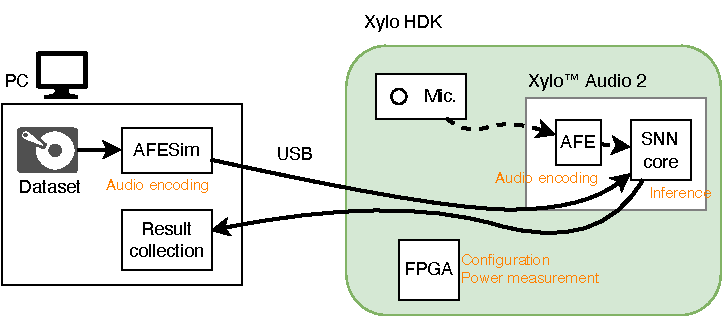
\includegraphics[width=\linewidth]{figures/xylo_system_overview.pdf}
    \vspace*{1cm}
    \end{subfigure}
    \hspace*{0.5cm}
    \begin{subfigure}{0.3\textwidth}
        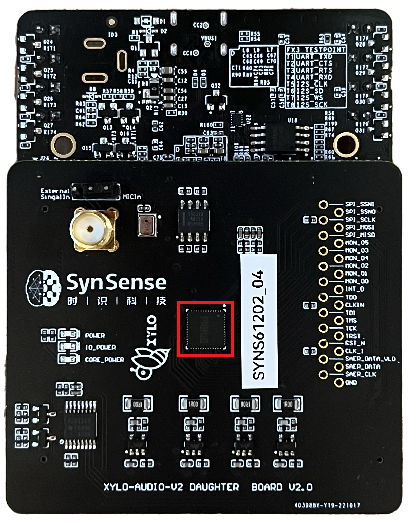
\includegraphics[width=\linewidth]{figures/xyloa2_hdk_fig.pdf}
    \end{subfigure}
        \caption{\secondrev{Left: An overview of the benchmarking system for the Xylo. A simulator of the analog encoding module is run on a PC and streamed to the SNN inference core via USB. After inference, outputs are routed back to the PC for classification. An on-board FPGA configures and records power of the Xylo components. Right: The Xylo\texttrademark Audio 2 hardware development kit (HDK), used as the SUT. The red outline marks the Xylo inference module. Figures taken, with permission, from Ke et al.~\cite{ke2024neurobenchdcase2020acoustic}}}
        \label{fig:xylo}
\end{figure}


\secondrev{\paragraph{CPU} The CPU baseline uses an Arduino Nano 33 BLE board, which runs preprocessing and inference on an ARM Cortex-M4F microcontroller running at 64MHz. All training and deployment uses Edge Impulse, a commercially developed ML-operations platform for tinyML~\cite{hymel2023edgeimpulsemlopsplatform}. The 1 second digital audio samples were converted into two-dimensional frames of Mel-filterbank energies (MFE), and inference uses a network with two convolution layers with batch normalization and max pooling. The trained model was quantized then compiled to an Arduino library using Edge Impulse EON compiler, which optimizes for memory and flash usage. Execution time is measured using on-chip timers from the Arduino, while power is measured using an external multimeter for total system power. Power was measured separately for idle, active pre-processing, and active inference by taking the average power over 60 seconds. The Arduino repeatedly computes over one sample loaded in memory, with a recording frequency of 3 Hz on a Keysight 34465A digital multimeter.}

\secondrev{\paragraph{Synsense Xylo} As shown in Figure~\ref{fig:xylo}, the Xylo baseline used a host PC to run a simulation of the analog pre-processing unit on the benchmark dataset, which was routed into the SNN core on the Xylo SUT. Accuracy is measured by performing a maximum on the output spikes of the SNN. The SNN on Xylo is a feedforward network with three hidden layers, where each layer is connected by synapses with varying time delays. Training is done using the open-source Rockpool toolchain~\cite{rockpool2019}. In order to amortize measurement overheads, power and execution time are measured over continuous streams of 10 seconds of audio, where the execution time result is divided by 10 and the power result is averaged over the duration. The measurements are made by the on-board FPGA, which operates at 12.5MHz and samples power at 1280 Hz. Accuracy is still measured on the 1-second samples. Full details are available in Ke et al.~\cite{ke2024neurobenchdcase2020acoustic}}


\subsubsection*{Quadratic Unconstrained Binary Optimization (QUBO)}
\begin{figure}[t]
    \centering
        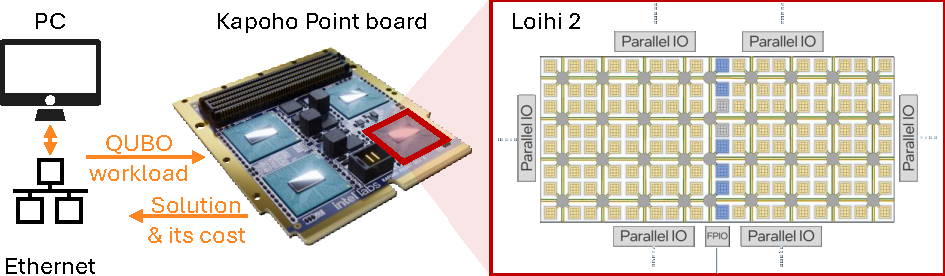
\includegraphics[width=0.85\linewidth]{figures/Loihi2_Benchmarking.pdf}
        \caption{\secondrev{A Kapoho Point board with Loihi 2 chips is connected to a host PC via ethernet. Shown here is a Kapoho Point board with 8 Loihi 2 chips, while the experiments were run on a board with 1 Loihi 2 chip. The QUBO workload is loaded onto the chip, and all processing happens on Loihi 2. On Loihi 2, the neuro-cores, in yellow, are arranged in two $8\times{}8$ grids and iteratively update the variables of the QUBO workload. Embedded CPUs, shown in blue, monitor the cost of the variable assignment. Six parallel IO ports enable 3D stacking of multiple chips for larger workloads than used here. An additional IO port provides the communication to the host PC. The energy and runtime measurements cover the computation of the Loihi 2 chip.}}
        \label{fig:loihi2}
\end{figure}


\secondrev{The processors ran repeatedly with five different initial variable assignments and seeds for different timeouts between $10^{-3}$ s to $10^{3}$ s, and for different workloads sizes of up to $1000$ variables. The neuromorphic algorithm is a parallelized version of simulated annealing that was running on a Kapoho Point board with one Loihi 2 chip, as shown in Figure~\ref{fig:loihi2}. The Loihi 2 board was controlled using Lava \texttt{0.8.0} and Lava Optimization \texttt{0.3.0}. For comparison with conventional hardware, two solvers were adopted based on simulated annealing and tabu search, as implemented in the D-Wave Samplers \texttt{v1.1.0} library \cite{dwavesamplers}. The library was compiled on Ubuntu \texttt{20.04.6 LTS} with GCC \texttt{9.4.0}  and Python \texttt{3.8.10}. CPU measurements were obtained on a machine with Intel Core i9-7920X CPU @ 2.90 GHz and 128GB of DDR4 RAM, using Intel SoC Watch for Linux OS \texttt{2023.2.0}. All details on the solvers, benchmarking routine, and results have been provided by Pierro et al.~\cite{pierro2024solvingquboloihi2}.
}


% \subsection*{System Track Metric Calculations}

% \TODO{Should move figure into the system track section, and probably delete this section from the Methods section}

% % \TODO{Need to verify this power measurement protocol - is it generally agreeable? I think it should note something about whether this is "wall-power" by power analyzer / power meter, or some internally generated power number. Also, do all submissions need to go through the high-level IR? it should be the goal that we have this tooling to aim for arbitrary workload execution, but it seems like the best performance would be achieved by skipping this and going straight to the low-level representation.}

% The correctness or accuracy metric of the systems is obtained in a partially controlled environment based on different representation levels (i.e., high-level and low-level IR in Figure \ref{fig:alg_system_harness}). The high-level consists of a common representation such as the Neuromorphic Intermediate Representation (NIR)~\cite{nir2023} or Lava~\cite{lava} aiming to unify spatio-temporal graphs describing the neuromorphic models to be deployed. Such high-level IR is then transformed into a more optimized representation (low-level IR) that is specific to the target hardware (e.g., sPyNNaker machine graph~\cite{spynnaker}). The low-level IR does not need to be shared between systems to enable hardware vendors to optimize their corresponding neural compilers and runtime execution environments towards achieving a good performance.  

% Throughput, and latency are relatively straightforward metrics to measure and calculate based on the performance of a given hardware platform. Hence, specific relevance is given to the power measurement protocol, as NeuroBench aims to standardize a fair approach to measure and compare different systems. Such protocol is exemplified for scalable systems as they offer presence in both edge- and server- based categories. However, this can be extrapolated to any other neuromorphic system. 

%     \begin{figure}[ht]
%             \centering
%             
\includegraphics[width=.95\textwidth]{figures/system_types.png}
%             \caption{Types of neuromorphic systems.}
%         \label{fig:system_types}
%     \end{figure}

% As presented in Figure~\ref{fig:system_types}, a neuromorphic system can have a single neuromorphic chip, or thousands of them in multi-chip PCBs connected in server setups. These systems commonly include but are not limited to high-speed links to enable fast connectivity within the mesh of neuromorphic processors, flash or any other external memory (e.g., DDR), built-in communication routers, supporting microcontrollers to manage the board, debugging ports (e.g., STLink, etc.), host ports (e.g., Ethernet, CAN, etc.), and a power management (PM) bus. The PM bus is of relevance for the system track metric calculation as it enables access to power consumed at different levels. The following steps exemplify the power characterization process:

% \begin{enumerate}
%     \item Create an SNN with parameters, weights, input spikes; map (partition) SNN to the target hardware and generate its experiment specification.
%     \item Initialize the target hardware.
%     \item Load the binaries (or equivalent) and parameters to the neuromorphic chip and start its cores to initialize them.
%     \item Load input data from the host to the hardware.
%     \item Execute the experiment on hardware triggered by the host. The experiment on the hardware runs standalone for a pre-defined time. This is the step in which the power is measured.
%     \item Read back the results from hardware to host.
%     \item Post-process the results and provide feedback to the user front end.
% \end{enumerate}

% Besides the previous steps, the following gathers some important aspects to establish a fair power management protocol between systems:

% \begin{itemize}
%     \item The power management bus should be connected to every single chip at the different levels of the system.
%     \item Each level should have a mechanism to reliably measure and report power.
%     \item When measurements rely on internal microcontrollers that are not easily accessible to the user, these should be characterized against controlled environments and disclosed within the submission to guarantee the validity of the readings. In complex systems, such characterization can be made for a single-board and extrapolated to the full scale, as the process is complex for supercomputer scales.
% \end{itemize}

% \subsection*{QUBO System Track Benchmark}
% Quadratic unconstrained binary optimization (QUBO) seeks binary variables

% \begin{equation}
% \mathbf{x} \in {0, 1}^n
% \end{equation}

% which optimize the cost function

% \begin{equation}
% C = \mathbf{x}^T \mathbf{Q} \mathbf{x}\ .
% \end{equation}

% The NeuroBench data set is generated by a workload generator and a set of parameters that specify matrices $\mathbf{Q}$. The set includes different workload sizes from $n=10$ binary variables to beyond 100,000s of variables to scale as NC systems mature. The matrix sparsity impacts the difficulty of the problem and is also provided by NeuroBench. For each size and sparsity, NeuroBench provides a set of random workloads for statistical testing.

% The metrics of the NeuroBench system track benchmark differ from benchmarks like MLPerf because NC systems are often designed to allow trading off not just performance and solution accuracy like ML systems, but also energy consumption. For example, neuromorphic systems can leave some of its cores idle to increase efficiency in trade off for less parallelism and thus reduced performance. In addition, NC systems are just maturating and thus quickly increase the size of supported networks. But the QUBO metrics differ also from other benchmarks of NeuroBench as the ground truth optimal solution of an NP-hard QUBO workload is intractable and cannot be straightforwardly determined by human labelling.

% The metrics of the NeuroBench QUBO benchmark account for these effects. The first metric is the maximum workload size supported, to make the benchmark inclusive to NC systems at all maturity levels. Energy efficiency and speed are the second and third metrics, measured by running multiple workloads of the largest supported workload size on the system without knowledge of the ground truth solution like other benchmarks for NP-hard combinatorial optimization \cite{taillard1993}. For each workload, the system is allowed to run for a specific time, and the cost function and energy consumption are recorded. This process is repeated across a range of timeouts. For each timeout, results are averaged over various random workloads of the same size and sparsity. The average accuracy at different timeouts can then be compared between neuromorphic systems and traditional hardware using paired statistics.  If the neuromorphic system outperforms traditional systems in time-to-solution, its energy consumption is then benchmarked separately at various timeouts. This is done by adjusting the system parameters to enhance energy efficiency, even if it means reducing accuracy. However, accuracy is kept just above iso-optimality compared to traditional hardware.  This approach allows to systematically benchmark the system on its maximum speed and its maximum energy efficiency.

% The neuromorphic system is measured against traditional hardware only on the largest workload size it supports to highlight the scaling benefits of neuromorphic computing. Still, researchers are urged to report numbers for all workload sizes supported by their NC system, to facilitate an inclusive comparison with neuromorphic systems that currently support only smaller problem sizes.

% The workload generator, the parameters specifying the workloads, the precise metrics, and initial state-of-the-art baselines on traditional hardware will be published in an upcoming paper and on GitHub.